\documentclass[../../FisicaTeorica.tex]{subfiles}


\begin{document}

\begin{comment}
\section{Lezione ?:\\ \large{Moto in campo a simmetria centrale 3D}}
\vspace{-1em}
\begin{center}
    \small{(3/12/2018)}
\end{center}
\end{comment}

\section{Potenziale centrale}
Occupiamoci ora dello studio di potenziali $U(r)$ a simmetria centrale, ossia che dipendono solo dalla distanza $r$ da un \textit{centro} fissato. Tale caso è infatti di grande rilevanza fisica, dato che ci permetterà di creare un modello dettagliato dell'\textit{atomo di idrogeno}.\\

Partiamo considerando, in generale,\marginpar{Moto di due particelle nel sdr del centro di massa} un sistema di due particelle distinguibili in $\bb{R}^3$ (che saranno protone ed elettrone nel caso dell'atomo di idrogeno) di massa rispettivamente $m_1$ e $m_2$, che interagiscono tra loro mediante un potenziale centrale $U(r)$, dove $r=|\vec{x}_1 - \vec{x}_2|$ è la distanza che le separa.\\
L'Hamiltoniana \textbf{classica} è data da:
\[
H=\frac{\vec{p}_1^{\,2}}{2m_1}+\frac{\vec{p}_2^{\,2}}{2m_2}+U(r)\qquad r=|\vec{x}_1 - \vec{x}_2|
\]
\textbf{Quantisticamente}, il sistema composto ha stati nel prodotto tensore degli spazi di Hilbert dei costituenti, ossia $\hs=L^2(\bb{R}^3, d^3x_1)\otimes L^2(\bb{R}^3, d^3x_2)$, e l'Hamiltoniana si ottiene sostituendo a $\vec{p}$  il relativo operatore quantistico $-i\hbar \nabla$ (in rappresentazione $\{\vec{x}\}$):
\[
H_{12} = -\frac{\hbar^2}{2m_1} \Delta_1 - \frac{\hbar^2}{2m_2} \Delta_2 + U(r)\qquad r=|\vec{x}_1 - \vec{x}_2|
\]
Per poter sfruttare la simmetria sferica del sistema, conviene riscrivere il tutto in funzione delle variabili $\vec{R}$ della posizione del Centro di Massa (CM), e del vettore $\vec{x}$ della distanza relativa tra le particelle:
\[
\vec{R}=\frac{m_1 \vec{x}_1 + m_2 \vec{x}_2}{m_1+m_2}; \quad \vec{x}=\vec{x}_1 -\vec{x}_2; \quad \hs \cong L^2(\bb{R}^3, d^3R) \otimes L^2(\bb{R}^3, d^3x)
\]
Da cui otteniamo:
\[
H_{12}=\underbrace{-\frac{\hbar^2}{2M}\Delta_R}_{H_R} \underbrace{- \frac{\hbar^2}{2m}\Delta_x + U(r)}_{H}\qquad M=m_1+m_2; \quad m=\frac{m_1 m_2}{m_1+m_2}
\]
dove riconosciamo in $m$ la \textit{massa ridotta} del sistema.\\
Esaminiamo i domini di autoaggiuntezza. $H_R$ è l'Hamiltoniana di una particella libera, di massa $M$ e centrata al CM, ed è definita in:
\[
D(H_R)=\{\psi\in L^2(\bb{R}^3, d^3R) \>|\> \vec{p}_R^{\,2} \tilde{\psi}(\vec{p}_R) \in L^2(\bb{R}^3, d^3 p_R)\}
\]
Per $H$ il caso è più delicato,\marginpar{Teorema di Kato-Rellich} ed è necessario fare ipotesi sulla natura del potenziale $U(r)$. Si può dimostrare (per il teorema di \textit{Kato-Rellich}), che se $U(r) \underset{r\to 0}{\sim} 1/r^\alpha$ per $\alpha < 3/2$ e $U(r) \underset{r\to\infty}{\sim}0$, con $U(r) \in L^2([0,1], r^2 dr)$ allora $H$ è autoaggiunto sullo stesso dominio del caso della particella libera, ossia:
\[
D(H) = \{\psi \in L^2(\bb{R}^3, d^3 x)\>|\> \vec{p}^{\,^2} \tilde{\psi}(\vec{p}) \in L^2(\bb{R}^3, d^3 p)\}
\]

Scriviamo allora l'equazione di Schr\"odinger stazionaria per il sistema:
\begin{align}
\left[-\frac{\hbar^2}{2M}\Delta_R - \frac{\hbar^2}{2m}\Delta_x + U(r)\right]\Psi(\vec{R},\vec{x})=\mathcal{E}_{tot}\Psi(\vec{R},\vec{x})
\label{eqn:schrodinger-centrale1}
\end{align}
Dato che i termini dell'Hamiltoniana agiscono dipendono rispettivamente solo da $\vec{R}$ o da $\vec{x}$, e mai da entrambi contemporaneamente, possiamo cercare una soluzione $\Psi(\vec{R},\vec{x})$ \textit{fattorizzata}:
\[
\Psi(\vec{R},\vec{x})=\varphi(\vec{R})\psi(\vec{x})
\]
Sostituendo in (\ref{eqn:schrodinger-centrale1}) otteniamo:
\[
-\frac{\hbar^2}{2M}(\Delta_R \varphi)\psi +\varphi\left[ -\frac{\hbar^2}{2m}\Delta_x \psi + U(r)\psi\right] = \mathcal{E}\varphi\psi
\]
Dividendo per $\varphi\psi$:
\[
\underbrace{-\frac{\hbar^2}{2M}\frac{\Delta_R \varphi}{\varphi}}_{\mathcal{E}_{CM}}+\underbrace{\left[
-\frac{\hbar^2}{2m} \frac{\Delta\psi}{\psi} + U(r)
\right]}_{\mathcal{E}} = \mathcal{E}_{tot}
\]
Spezzando l'energia in $\mathcal{E}_{tot}=\mathcal{E}+\mathcal{E}_{CM}$, otteniamo due equazioni distinte. In particolare, la parte che deriva da $H_R$ genera l'equazione di Schr\"odinger di una particella libera, che sappiamo trattare:
\begin{align*}
-\frac{\hbar^2}{2M}\Delta_R\varphi = \mathcal{E}_{CM}\varphi
\end{align*}
Occupiamoci allora della parte relativa ad $H$, che è ben più interessante data la presenza del potenziale centrale $U(r)$.\\

Poiché $U(r)$ ha simmetria sferica,\marginpar{Simmetria sferica di $H$} notiamo che $H$ è invariante per rotazioni:
\[
\exp\left(-i\frac{\varphi}{\hbar}\vec{L}\cdot\vec{n}\right) H \exp\left(i\frac{\varphi}{\hbar}\vec{L}\cdot \vec{n}\right) = H \Rightarrow [H, \vec{L}]=0; \quad [H,\vec{L}^2]=0
\]
Pertanto $H$, $\vec{L}^2$, $L_3$ sono tre osservabili compatibili tra loro, e perciò ammettono una base di autoket comuni $\ket{\mathcal{E}, l, m}$. Spezziamo allora il problema in parte \textit{radiale} e \textit{angolare}, tramite l'isomorfismo \q{delle coordinate sferiche} $L^2(\bb{R}^3,d^3x) \cong L^2(\bb{R}_+, r^2 dr) \otimes L^2(S^2, d\Omega)$.\\
Sappiamo che in $L^2(S^2, d\Omega)$, $\{\vec{L}^2, L_z\}$ costituiscono un ICOC.\marginpar{Autoket comuni $\ket{\mathcal{E}, l, m}$} Sapremo allora che $\{H,\vec{L}^2, L_3\}$ è un ICOC per il sistema \textit{ridotto} con hamiltoniana $H$ se, una volta fissati i valori di $\vec{L}^2$ e $L_z$, tramite i loro autovalori $l$ e $m$, l'hamiltoniana $H(l,m)$ in $L^2(\bb{R}_+, r^2 dr)$ risulta avere uno \textbf{spettro non degenere}. In altre parole, vogliamo verificare che fissati $l$ e $m$, per un dato $\mathcal{E}$ ci sia un \textit{solo} autoket comune $\ket{\mathcal{E}, l, m}$.\\

Dimostriamolo. Partiamo riscrivendo $\vec{L}^2$ in termini di $\vec{P}^2$ (che compare in $H$), in modo da poter cercare agilmente gli autostati comuni $\ket{\mathcal{E}, l, m}$.
Con la convenzione di Einstein, sfruttiamo l'identità:
\begin{align}
\epsilon_{ijk}\epsilon_{ilm}=\delta_{jl}\delta_{km}-\delta_{jm}\delta_{kl}
\label{eqn:identity-civita}
\end{align}

Per cui:
\begin{align}\nonumber
\vec{L}^{\,2} &= L_i L_i =(\epsilon_{ijk}X_j P_k)(\epsilon_{ilm} X_l P_m) \underset{(\ref{eqn:identity-civita})}{=} (\delta_{jl}\delta_{km}-\delta_{jm}\delta_{kl})X_j P_k X_l P_m =\\\nonumber
&\underset{(a)}{=} \hlc{Yellow}{\delta_{jl}}\hlc{SkyBlue}{\delta_{km}}\hlc{Yellow}{X_j}(\hlc{Yellow}{X_l }\hlc{SkyBlue}{P_k} + \underbrace{[P_k, X_l]}_{-i\hbar\delta_{kl}})\hlc{SkyBlue}{P_m} - \delta_{jm}\delta_{kl} X_j P_k (P_m X_l + \underbrace{[X_l, P_k]}_{i\hbar \delta_{lm}}) =\\\nonumber
&\underset{(b)}{=} \hlc{Yellow}{\vec{X}^{\,2}}\hlc{SkyBlue}{\vec{P}^{\,2}} - i\hbar (\vec{X}\cdot \vec{P}) - (\vec{X}\cdot\vec{P})\> \underbrace{(\vec{P}\cdot \vec{X})}_{\vec{X}\cdot \vec{P}-3i\hbar} -i\hbar (\vec{X}\cdot\vec{P})=\\\nonumber
&\underset{(c)}{=}\vec{X}^{\,2}\vec{P}^{\,2} \hlc{ForestGreen}{- i\hbar \vec{X}\cdot\vec{P} }- (\vec{X}\cdot \vec{P})^2\hlc{ForestGreen}{+3i\hbar \vec{X}\cdot\vec{P}-i\hbar \vec{X}\cdot\vec{P}}=\\ \label{eqn:Lquadro_Pquadro}
&=\vec{X}^{\,2}\vec{P}^{\,2}-(\vec{X}\cdot\vec{P})^2 \hlc{ForestGreen}{+ i\hbar \vec{X}\cdot\vec{P}}
\end{align}
In (a) abbiamo usato i commutatori per portare le $X_j$ e $X_l$ \textit{vicine}, e analogamente $P_k$ e $P_m$, in modo da ottenere i successivi quadrati e prodotti scalari.\\
In (b), espandendo i prodotti, notiamo che\footnote{Si può pensare a una $\delta_{jm}$ come tale da \q{identificare} gli indici. Il prodotto di più delta identifica tra loro più indici contemporaneamente. Un trucco per risolvere le uguaglianze è la \q{semplificazione} data dalla contrazione di indici uguali confinanti $\delta_{k\bcancel{l}}\delta_{\bcancel{l}m}=\delta_{km}$. Si ricorda inoltre che la delta di Kronecker è \textit{simmetrica}: $\delta_{km}=\delta_{mk}$.}:
\begin{align*}
\delta_{jl}\delta_{km}\delta_{kl}&=\delta_{jl}\delta_{lm}=\delta_{jm}
\end{align*}
E quindi, per esempio:
\begin{align*}
\delta_{jl}\delta_{km}\delta_{kl} X_j P_m =\delta_{jm}X_jP_m =X_j P_j =\vec{X}\cdot \vec{P}
\end{align*}
Analogamente vale:
\begin{align*}
\delta_{jm}\delta_{kl}\delta_{lm}&=\delta_{jm}\delta_{km} = \delta_{jk}
\end{align*}
In (c) \q{invertiamo} il prodotto scalare tramite i commutatori. In notazione di Einstein, e calcolando alla fine le somme:
\begin{align*}
\vec{X}\cdot \vec{P} = X_i P_i = [X_i, P_i] + P_i X_i = 3i\hbar + \vec{P}\cdot \vec{X} \Rightarrow  \vec{P}\cdot \vec{X} = \vec{X}\cdot\vec{P} - 3i\hbar
\end{align*}

Invertendo la (\ref{eqn:Lquadro_Pquadro}) otteniamo $\vec{P}^2$ in termini di $\vec{L}^2$:
\begin{align}
\vec{P}^{\,2} =\vec{X}^{-2} [(\vec{X}\cdot \vec{P})^2+\vec{L}^{\,2}-i\hbar \vec{X}\cdot\vec{P}]
\label{eqn:Pquadro_Lquadro}
\end{align}
che è pronto per essere sostituito in $H$. Prima di farlo, però, conviene passare in \textit{coordinate sferiche}. Facciamolo un termine alla volta, ricordando il passaggio da $\vec{\nabla}=(\partial_x, \partial_y, \partial_z)^t$ a $(\partial_r, \partial_\theta, \partial_\varphi)^t$ visto in (\ref{eqn:relazione_inversa}).
\begin{align*}
\vec{X}\cdot \vec{P} &= -i\hbar \vec{x}\cdot \vec{\nabla} = -i\hbar r \frac{\partial}{\partial r}\\
\end{align*}
Dato che:
\begin{align*}
\vec{x}\cdot\vec{\nabla} &= r\sin\theta\cos\varphi \left(\sin\theta\cos\varphi \frac{\partial}{\partial r} + \cancel{\frac{1}{r}\cos\theta\cos\varphi\frac{\partial}{\partial \theta}} - \bcancel{\frac{\sin\varphi}{r\sin\theta}\frac{\partial}{\partial \varphi}}\right)+\\
&+r\sin\theta\sin\varphi \left(\sin\theta\sin\varphi \frac{\partial}{\partial r} + \cancel{\frac{1}{r}\cos\theta\sin\varphi\frac{\partial}{\partial \theta}} + \bcancel{\frac{\cos\varphi}{r\sin\theta}\frac{\partial}{\partial \varphi}}\right)+\\
&+r\cos\theta \left(\cos\theta \frac{\partial}{\partial r} -\cancel{\frac{\sin\theta}{r}\frac{\partial}{\partial \theta}}\right) =\\
&=r[\sin^2\theta\cos^2\varphi + \sin^2\theta\sin^2\varphi + \cos^2\theta] \frac{\partial}{\partial r} = r\frac{\partial}{\partial r}
\end{align*}
Ricaviamo poi:
\begin{align*}
(\vec{X}\cdot \vec{P})^2 = \left(-i\hbar r\frac{\partial}{\partial r}\right)\left(-i\hbar r \frac{\partial}{\partial r}\right) = -\hbar^2 r \frac{\partial}{\partial r} r \frac{\partial}{\partial r}
\end{align*}
E sostituendo tutto ciò in (\ref{eqn:Pquadro_Lquadro}) otteniamo:
\begin{align}
\vec{P}^{\,2} &= \frac{1}{r^2} \left[ -\hbar^2 r \frac{\partial}{\partial r} {r \frac{\partial }{\partial r}} + \vec{L}^{\,2} - \hbar^{2} r \frac{\partial}{\partial r}\right]=\frac{1}{r^2}\left[-\hbar^2 r\left(\hlc{Yellow}{\frac{\partial}{\partial r}r\frac{\partial}{\partial r}+\frac{\partial}{\partial r}}\right) + \vec{L}^2 \right]
\label{eqn:Pquadro_Lquadro2}
\end{align}
Possiamo semplificare ulteriormente questa espressione, notando che:
\begin{align*}
r\frac{\partial}{\partial r} = \frac{\partial}{\partial r}r-1
\end{align*}
Come tutte le uguaglianze di operatori, il modo corretto per dimostrarla sta nell'applicarla ad una generica funzione $f(r)$:
\begin{align*}
r\frac{\partial}{\partial r} f(r)&= r f'(r)\\
\left(\frac{\partial}{\partial r}r-1\right)f(r)&=\frac{\partial}{\partial r}(rf(r))-f(r) = f(r)+rf'(r)-f(r)=rf'(r)
\end{align*}
Il termine evidenziato in (\ref{eqn:Pquadro_Lquadro2}) diviene perciò:
\begin{align*}
\frac{\partial}{\partial r}r\frac{\partial}{\partial r} + \frac{\partial}{\partial r} = \frac{\partial}{\partial r}\left(\frac{\partial}{\partial r}r-1\right)+\frac{\partial}{\partial r}=\frac{\partial^2}{\partial r^2}r-\frac{\partial}{\partial r} + \frac{\partial}{\partial r} =\frac{\partial^2}{\partial r^2}r
\end{align*}
E infine otteniamo:
\begin{align}
\vec{P}^{\,2}=\frac{1}{r^2}\left[\hlc{Yellow}{-\hbar^2r \frac{\partial^2}{\partial r^2}r}+ \vec{L}^2 \right]
\label{eqn:Pquadro_Lquadro3}
\end{align}
Sostituendo nell'Hamiltoniana $H$, giungiamo a:
\begin{align}
H=\frac{1}{2m}\left[\hlc{Yellow}{-\frac{\hbar^2}{r}\frac{\partial^2}{\partial r^2}r} +\frac{\vec{L}^2}{r^2}\right]
\label{eqn:hamiltoniana-centrale}
\end{align}

Per ottenere una qualche\marginpar{Confronto con il caso classico} intuizione sulla natura \textit{fisica} del termine evidenziato confrontiamo quanto abbiamo ottenuto con il caso classico.\\
Come è noto dai corsi di Fisica, un punto di massa $m$ posto in un potenziale centrale $U(r)$ (che ipotizziamo centrato nell'origine) sperimenta una forza $\vec{F} = -\vec{\nabla}U(r)$ diretta verso $O$. Il momento torcente rispetto al polo $O$ è allora nullo: $\vec{\tau}=\vec{r}\times \vec{F} =0$, e perciò il momento angolare è costante:
\begin{align*}
\frac{d\vec{L}}{dt}=\vec{\tau} =0
\end{align*}
Scomponendo allora l'energia $\mathcal{E}$ della particella nei contributi dovuti al moto $v_r \hat{r}$ verso $O$, e quello $v_\perp \hat{\theta}$ ad esso perpendicolare, si ha:
\begin{align*}
\mathcal{E} =\frac{1}{2}mv_r^2 + \frac{1}{2}mv_\perp^2 + U(r) = \frac{p^2}{2m} + U(r)
\end{align*}
dove $\vec{p}=m\vec{v}$ è il momento della particella. Possiamo riscrivere $\mathcal{E}$ utilizzando il momento angolare $|\vec{L}|=mrv_\perp$, e introducendo il \textit{momento radiale} $p_r = m v_r$:
\begin{align}
\mathcal{E} = \frac{1}{2m}\left(p_r^2 + \frac{L^2}{r^2}\right) \Rightarrow  p^2=p_r^2 + \frac{1}{r^2}L^2
\label{eqn:momento-radiale-classico}
\end{align}

Confrontando (\ref{eqn:momento-radiale-classico}) con (\ref{eqn:Pquadro_Lquadro3}) scopriamo che il termine evidenziato è proprio il quadrato del \textit{momento radiale} $P_r^2$.

\begin{expl}
\textbf{Nota}: il momento radiale $P_r$ non si ottiene semplicemente dalla \q{radice quadrata} di $P_r^2$, ma è dato da:
\begin{align*}
P_r = -i\hbar\frac{1}{r}\frac{\partial}{\partial r} r
\end{align*}
Infatti:
\begin{align*}
P_r^2=\left(-i\hbar \frac{1}{r}\frac{\partial}{\partial r} \bcancel{r}\right)\left(-i\hbar \frac{1}{\bcancel{r}}\frac{\partial}{\partial r}r\right) = -\hbar^2\frac{1}{r}\frac{\partial^2}{\partial r^2} r
\end{align*}
\end{expl}

Definiamo allora il \textbf{momento radiale}\marginpar{Momento radiale quadro $P_r^2$ e sua autoaggiuntezza} $P_r = -i\hbar \frac{1}{r}\frac{\partial}{\partial r} r$ in $L^2(\bb{R}_+, r^2 dr)$, e mostriamo che il suo quadrato $P_r^2 = -\hbar^2 \frac{1}{r^2} \frac{\partial^2}{\partial r^2} r$ è autoaggiunto nel dominio:
\[
D(P_r^2) = \{
\psi \in L^2(\bb{R}_+, r^2 dr),\>\text{$\psi$ regolari con $\lim_{r\to 0} r\psi(r)=0$}
\}
\]
Infatti, prendendo:
\[
\varphi \in D((P^2_r)^\dag), \> \psi \in D(P_r^2)
\]
e calcolando gli elementi di matrice, si ha che:
\begin{comment}
\begin{align*}
\left(\varphi, \frac{P_r^2 \psi}{\hbar^2}\right) &=\int_0^\infty \varphi*(r) \frac{1}{r}\frac{\partial^2}{\partial r^2}(r\psi(r)) r^2\,dr \underset{\text{int parti}}{=}
(r\varphi^*)\frac{\partial}{\partial r}(r\psi)\Big|_{0}^{+\infty} - \int_0^{\infty}\frac{\partial}{\partial r}(r\varphi^*)\frac{\partial}{\partial r}(r\psi) dr =\\
&\underset{\text{parti}}{=}-r\varphi^* \frac{\partial}{\partial r}(r\psi)(0) - \bcancel{\frac{\partial}{\partial r}(r \varphi^*) (r\psi)\Big|_0}^{\infty} + \int_0^\infty \frac{\partial^2}{\partial r^2} (r\varphi^*) (r\psi) dr=\\
&=\hlc{ForestGreen}{-r\varphi^* \frac{\partial}{\partial r}(r\psi)(0)} + \frac{\partial}{\partial r}(r\varphi^*)r\underbrace{\psi(0)}_{\substack{=0\\\psi \in D(P_r^2)}} + \left(\frac{P^2_r}{-\hbar^2}\varphi, \psi\right)
\end{align*}
\end{comment}
\begin{align}
\left(\varphi, \frac{P_r^2 \psi}{-\hbar^2}\right) = \int_0^{+\infty} \hlc{Yellow}{r^2 dr}\, \varphi^* \frac{1}{r} \frac{\partial^2}{\partial r^2} (r\psi(r))
\label{eqn:elemento-matrice-Pquadro}
\end{align}
dove l'integrazione su $r^2 dr$ deriva dalla componente radiale della misura delle coordinate sferiche:
\begin{align*}
dV =\hlc{Yellow}{r^2 dr} \land \sin\theta d\theta \land d\varphi
\end{align*}
Integriamo per parti due volte l'espressione (\ref{eqn:elemento-matrice-Pquadro}), per esempio tramite il \textit{metodo tabulare}:
\begin{table}[H]
\centering
\begin{tabular}{@{}rr@{}}
\toprule
$r\varphi^*$ & $\partial_{r^2}(r\psi)$\\ \midrule
$-\partial_r (r\varphi^*)$ & $\partial_r (r\psi)$\\
$\partial_{r^2}(r\varphi^*)$ & $r\psi$\\
\bottomrule
\end{tabular}
\caption{Metodo tabulare per l'integrazione per parti}
\end{table}
Da cui:
\begin{align}
(\ref{eqn:elemento-matrice-Pquadro})=(r\varphi^*)\frac{\partial}{\partial r}(r\psi)\Big|_0^{+\infty} -\frac{\partial}{\partial r}(r\varphi^*)r\psi\Big|_0^{+\infty} + \int_0^{+\infty}dr\,(r\psi) \frac{\partial^2}{\partial r^2}(r\varphi^*)
\label{eqn:elemento-matrice-Pquadro2}
\end{align}
Riconosciamo nell'ultimo termine il prodotto scalare tra $P_r^2/-\hbar^2$ applicato a $\varphi^*$ e $\psi$, come desiderato. Inoltre, essendo $\varphi, \psi \in L^2$, sappiamo che $\varphi^*(+\infty)\to 0$, e $\psi(+\infty)\to 0$, e perciò:
\begin{align*}
(\ref{eqn:elemento-matrice-Pquadro2})=-\hlc{ForestGreen}{\left(r\varphi^*\frac{\partial}{\partial r}(r\psi)\right)(0)} +\hlc{Yellow}{ \left(\frac{\partial}{\partial r}(r\varphi')r\psi\right)(0)} + \left(\frac{P_r^2}{-\hbar^2}\varphi,\psi\right)
\end{align*}
Poiché $\psi \in D(P_r^2)$, vale $r\psi \xrightarrow[r\to0]{}0$, e perciò il termine giallo è nullo. Se vogliamo che $P_r^2$ coincida con il suo aggiunto, dobbiamo imporre che anche il termine evidenziato si annulli. Ma non abbiamo alcuna condizione su $\partial_r(r\psi)$, e quindi dobbiamo imporre per forza:
\[
\lim_{r \to 0} r\varphi(0) = 0
\]
Osserviamo che in questo modo si impone la stessa condizione sia per il dominio di $P_r^2$ che per quello del suo aggiunto $(P_r^2)^\dag$ e aggiunto, da cui:
\[
D(P_r^2) = D((P_r^2)^\dag)
\]
Ciò, assieme all'identità appena verificata per gli elementi di matrice:
\begin{align*}
\left(\varphi, \frac{P_r^2 \psi}{-\hbar^2}\right)=\left(\frac{P_r^2}{-\hbar^2}\varphi,\psi\right)
\end{align*}
dimostra l'autoaggiuntezza di $P_r^2$.\\

L'Hamiltoniana \textit{ridotta} $H$ del sistema è allora:
\[
H = \frac{1}{2m}\left[P_r^2 + U(r) + \frac{\vec{L}}{r^2} (\theta,\varphi)\right]\quad \lim_{r\to 0} r\psi(r) = 0
\]
Scriviamo quindi l'equazione di Schr\"odinger stazionaria:
\begin{align}
\frac{1}{2m}\left[\vec{P}_r^2 + \frac{\vec{L}^2}{r^2}(\theta,\varphi) + U(r)\right] \psi(r,\theta,\varphi) = \mathcal{E}\psi(r,\theta,\varphi)
\label{eqn:schrody-centrale2}
\end{align}
Vogliamo ora trovare esplicitamente gli autoket comuni $\ket{\epsilon, l, m}$.
Notiamo che termini radiali e angolari sono \textit{separati}, e ciò suggerisce di cercare soluzioni \textit{fattorizzabili}. Di queste, abbiamo già ricavato la forma degli autoket angolari $\ket{l,m}$, che sono proprio le armoniche sferiche: $Y_l^m(\theta,\varphi)$. Perciò fattorizziamo le autofunzioni comuni $\psi$ come:
\[
\psi_{\epsilon l m}(r,\theta,\varphi) = h_{\epsilon l m}(r) Y^m_l(\theta,\varphi)
\]
Data la simmetria sferica del sistema, ci aspettiamo che l'autofunzione radiale $h(r)$ \textit{non} dipenda dall'autovalore $m$ - se così fosse avremmo una direzione ($\hat{z}$) distinguibile dalle altre. In effetti, $H$ dipende solo da operatori radiali e da $\vec{L}^2$, e non da $L_3$. Esplicitamente, se proviamo ad abbassare/alzare gli autovalori di $m$ in $\psi$ tramite $L_\pm$, $h_{\epsilon lm}$ resta invariata:
\begin{align*}
L_\pm \psi_{\epsilon l m}(\vec{r})&=\hbar \sqrt{l(l+1)-m(m\pm 1)}\psi_{\epsilon l, m\pm 1}(\vec{r})\\
L_\pm \psi_{\epsilon l m}(\vec{r}) &= h_{\epsilon l m}(r)L_\pm Y_l^m(\theta,\varphi)=\hbar \sqrt{l(l+1)-m(m\pm 1)}h_{\epsilon l m}(r) Y_l^{m\pm1}(\theta,\varphi)
\end{align*}
E perciò $h_{\epsilon l m}(r) = h_{\epsilon l, m\pm 1}(r)$. In altre parole, $h$ è indipendente dall'indice $m$, che perciò possiamo rimuovere. Giungiamo allora a:
\begin{align}
\psi_{\epsilon l m}(r,\theta,\varphi)=h_{lm}(r) Y_l^m(\theta,\varphi)
\label{eqn:soluzione_fattorizzata_centrale}
\end{align}
Per cui valgono le equazioni agli autovalori:
\begin{align*}
H \ket{\epsilon, l ,m} = \mathcal{E}_{\epsilon l}\ket{\epsilon, l,m} \quad \vec{L}^2 \ket{\epsilon, l,m} = \hbar^2 l(l+1) \ket{\epsilon, l,m} \quad L_3 \ket{\epsilon,l,m} = \hbar m \ket{\epsilon,l,m}
\end{align*}
Ci rimane solo da trovare un'espressione esplicita per $h_{\epsilon l}(r)$, per cui è però necessario definire la forma di $U(r)$. Occupiamoci per il momento di trovare alcune proprietà generali. Sostituendo (\ref{eqn:soluzione_fattorizzata_centrale}) in (\ref{eqn:schrody-centrale2}) e svolgendo le equazioni agli autovalori, giungiamo a:
\begin{align}
\left[ - \frac{\hbar^2}{r}\frac{d^2}{dr^2} \hlc{Yellow}{r} + \frac{\hbar^2 l (l+1)}{r^2}-2m(\mathcal{E}-U(r)\right] h_{\epsilon l}(r) = 0
\label{eqn:autoval_psi}
\end{align}
Possiamo semplificare tale equazione includendo l'$r$ evidenziato nella funzione, e cioè definendo:
\[
\chi_{\epsilon l}(r) = rh_{\epsilon l}(r)
\]
Dalla condizione $\lim_{r\to 0}r \psi(r) = 0$ abbiamo:
\[
\chi_{\epsilon l } = 0
\]
Perciò la (\ref{eqn:autoval_psi}) diviene:
\begin{align}
\frac{d^2 \chi_{\epsilon l}(r)}{dr^2} + \left[
\frac{2m}{\hbar^2}(\mathcal{E}-U(r)) - \hlc{ForestGreen}{\frac{l(l+1)}{r^2}}\right] \chi_{\epsilon l}(r) =\ 0
\label{eqn:equazione_radiale}
\end{align}
La condizione di normalizzazione si riduce a:
\[
\infty > \int_0^\infty |h_{\epsilon l}(r)|^2 r^2 dr =\int_0^\infty |\chi_{\epsilon l}(r)|^2\,\hlc{SkyBlue}{dr}
\]
Notiamo allora che introdurre $\chi_{\epsilon l}(r)$ permette di trattare un problema \textit{radiale} (in coordinate sferiche) come uno unidimensionale \textit{cartesiano} in $L^2(\bb{R}_+, \hlc{SkyBlue}{\bm{dr}})$. Lo possiamo vedere esplicitamente \q{inglobando} il termine evidenziato in verde nella (\ref{eqn:equazione_radiale}) in un potenziale \textit{effettivo} a $l$ fissato:
\begin{align*}
U^{\mathrm{eff}}_l(r) \equiv U(r) + \frac{\hbar^2}{2m}\frac{l(l+1)}{r^2}
\end{align*}
dove il termine aggiuntivo è analogo a quello dell'\textit{energia centrifuga} del caso classico, che funge da \q{barriera} che impedisce a una particella con momento angolare non nullo (e quindi $l\neq 0$) di precipitare sull'origine, dove violerebbe la conservazione del momento angolare.
\begin{figure}[H]
\centering
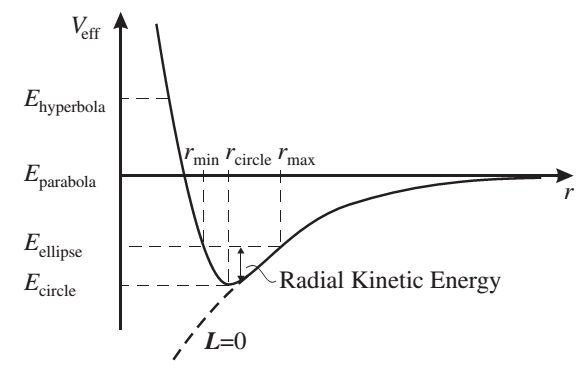
\includegraphics[scale=0.5]{Immagini/3_12/image001.png}
\caption{Andamento qualitativo del potenziale effettivo $U^{\mathrm{eff}}_l(r)$}
\end{figure}
Così facendo, otteniamo l'equazione:
\begin{align*}
\left[-\frac{\hbar^2}{2m}\frac{d^2}{dr^2} + U_l^{\mathrm{eff}}(r)\right]\chi_{\epsilon l}(r)=\mathcal{E}_{\epsilon l} \chi_{\epsilon l}
\end{align*}
che è l'equazione di Schr\"odinger stazionaria per una particella confinata in $\mathbb{R}_+$ in un potenziale unidimensionale\footnote{Ponendo $U_{l}^{\mathrm{eff}}(r)=+\infty$ per $r<0$ possiamo ricondurre il problema a tutto $\bb{R}$.}\\
Di tale sistema, almeno qualitativamente, sappiamo già dire tutto. Facendo riferimento alla sezione \ref{sec:potenziali_generici}, poiché $U_l^\mathrm{eff}(0)=+\infty$ (e infatti si ha $\chi(0)=0$) il moto avviene in una regione semilimitata, ossia solo per $r>0$. Ne segue che, fissati $l$ e $m$, lo spettro $\sigma(H)$ è sempre non degenere. Ma questo è proprio quello che volevamo dimostrare: possiamo perciò affermare che $\{H, \vec{L}^{\,2},L_3\}$ costituisca un ICOC per il sistema considerato.\\
A seconda del valore di $\mathcal{E}$ si presentano allora due casi:
\begin{itemize}
\item $V_{\min} < \mathcal{E} < 0$: le soluzioni $\chi_{\epsilon l}(r) \in L^2(\bb{R})$, e perciò devono soddisfare la condizione $\chi(0)=0$. Ciò corrisponde allo \textit{spettro discreto} degli \textit{stati legati}.
\item $0 < \mathcal{E} < +\infty$: le soluzioni non sono più in $L^2$, ossia non sono più \q{fisiche} - e ciò corrisponde allo \textit{spettro continuo} del sistema. In tal caso avremo solo che $\psi=h_{\epsilon l}(r)Y_l^m(\theta,\varphi) \in \mathcal{S}'(\bb{R}^3)$.
\end{itemize}

\subsection{Particella libera in coordinate sferiche}
Per proseguire oltre è necessario specificare l'espressione del potenziale centrale $U(r)$. Partiamo dal caso più semplice, in cui $U(r) \equiv 0$, che non è altro che la riscrittura delle funzioni d'onda di una particella libera in coordinate sferiche. Dato che deve essere $\mathcal{E} > V_{\min}=0$, ci aspettiamo uno \textit{spettro continuo} (dato che, del resto, la particella non è confinata), e \textit{nondegenere}, come visto nella precedente discussione.\\
Infatti (\ref{eqn:equazione_radiale}) diviene:
\begin{align}
\left[\frac{d^2}{dr^2}-\frac{l(l+1)}{r^2} + \frac{2m}{\hbar^2}\mathcal{E}\right] \chi_{\epsilon l}(r) = 0
\label{eqn:potenziale_centrale_nullo}
\end{align}
Per risolverla, supponiamo che $\chi_{\epsilon r}(r)$ sia sufficientemente regolare da consentire un'espansione in serie di potenze attorno all'origine, dove il termine dominante sarà $r^\alpha$ per un certo $\alpha > 0$. 
\begin{equation}
\chi_{\mathcal{E}l}(r) \underset{r \to 0}{\sim} r^\alpha \qquad \alpha > 0
\label{eqn:punto_zero}
\end{equation}
Sostituiamo in (\ref{eqn:potenziale_centrale_nullo}) per esaminare l'equazione nel \textit{punto singolare} per $r\to 0$, dove l'\textit{energia centrifuga} domina e quindi trascuriamo il termine con $\mathcal{E}$:
\begin{align}\nonumber
\left[\frac{d^2}{dr^2}-\frac{l(l+1)}{r^2}\right] \chi_{\mathcal{E}l}(r)&=0\\
\alpha(\alpha -1 )r^{(\alpha-2)} - l(l+1)r^{\alpha-2}&=0 \label{eqn:asintoto-origine}\\
\Rightarrow \alpha^2 - \alpha - l^2 - l = 0 \Rightarrow \alpha_{1,2} = l+1, -l \span \nonumber
\end{align}
In principio, $r^{l+1}$ e $r^{-l}$ sono due soluzioni possibili. Di queste, tuttavia, $r^{-l}$ è \textit{spuria}, ed è introdotta dal fatto che, nel passaggio a coordinate sferiche, si ha una singolarità all'origine (dove la matrice jacobiana è singolare). Possiamo scartarla osservando che:
\begin{itemize}
\item Per lo \textit{spettro discreto} deve essere $\chi_{\epsilon l}(0) = 0$, e $r^{-l} \neq 0$ (o addirittura diverge) per $l\geq 0$.
\item Per lo \textit{spettro continuo}, deve essere $\psi=h\chi \in \mathcal{S}'$, e perciò non possiamo immediatamente scartare $r^{-l}$. Notiamo però che per $l>0$ la $\psi$ non è normalizzabile in coordinate sferiche, mentre per $l=0$ si ha che $\chi_{\epsilon 0}\sim1$, da cui $h=\chi/r \sim r^{-1}$, e dato che $Y_0 \sim 1$, la $\psi = hY \sim r^{-1}$. Ma tale $\psi$ non può essere (nemmeno in $\mathcal{S}'$) la funzione d'onda di uno stato stazionario, poiché non verifica l'equazione di Schr\"odinger. Infatti, il suo laplaciano (che compare nell'equazione stazionaria) è una $\delta$:
\begin{align*}
\Delta(hY)\sim \Delta \frac{1}{r} = \delta^{(3)}(\vec{x})
\end{align*}
che non viene \textit{cancellata} da alcun altro termine dell'equazione, dato che il potenziale $U(r)$ è ipotizzato regolare a meno di salti.
\end{itemize}
Escludendo il caso $r^{-l}$, giungiamo a:
\begin{align*}
\chi_{\epsilon l} (r) \underset{r \to 0}{\sim} r^{l+1}
\end{align*}

Notiamo\marginpar{Estensione a potenziali \q{coulombiani}} che questo risultato si estende anche agli $U(r)$ per cui $r^2 U(r) \underset{r\to 0}{\sim} 0$ (come nel caso del potenziale coulombiano) cosicché $U(r)$ è trascurabile rispetto a $d^2/dr^2$ e $l(l+1)/r^2$ per $r\to 0$, e perciò l'espressione (\ref{eqn:asintoto-origine}) da cui siamo partiti vale senza modifiche.\\

Per trovare esplicitamente le autofunzioni radiali partiamo esaminando il caso di $l=0$, e cerchiamo di costruire tutto il resto partendo da lì. In tal caso, la (\ref{eqn:potenziale_centrale_nullo})
diviene l'equazione differenziale di un oscillatore armonico:
\begin{align}
\left[\frac{d^2}{dr^2} + k^2 \right] \chi_{\mathcal{E}0} (r) = 0 \qquad k = \sqrt{\frac{2m\mathcal{E}}{\hbar^2}}
\label{eqn:pot-centrale-nullo-differenziale}
\end{align}
Che ha due soluzioni indipendenti:
\begin{align*}
\chi_{\epsilon 0}(r)=
\begin{cases}
\sin(k r) \Rightarrow  h_{\epsilon 0}=\frac{\sin(kr)}{r} \quad \chi_{\epsilon 0}(0) = 0\\
\cos(kr)  \Rightarrow  h_{\epsilon 0} = \frac{\cos(kr)}{r} \quad \chi_{\epsilon 0}(0) \neq 0
\end{cases}
\end{align*}
Per cui la condizione in $r=0$ è soddisfatta solo dalla prima soluzione, che è l'unica accettabile: del resto sappiamo che gli autostati radiali sono \textit{nondegeneri}.\\

Per $l>0$ sappiamo che $\chi_{\epsilon l} \sim r^{l+1}$ attorno all'origine, e perciò $h=\chi/r$ sarà, in generale, il prodotto tra $r^l$ e una opportuna funzione $h_{kl}(r)$ che \textit{non ne modifichi} l'andamento nei pressi di $0$: 
\begin{equation}
h_{\epsilon l}(r) = r^l h_{kl}(r)\qquad h_{kl}(r) \xrightarrow[r \to 0]{} \text{cost}\neq 0
\label{eqn:h_lgrandi}
\end{equation}
Sostituendo (\ref{eqn:h_lgrandi}) nell'equazione differenziale troviamo una condizione che deve rispettare la $h_{kl}(r)$, e che ci permetterà di determinarla:
\begin{align*}0 &=
\left[\frac{d^2}{dr^2} + k^2 -\frac{l(l+1)}{r^2}\right] \underbrace{rh_{\epsilon l}}_{\chi_{\epsilon l}}\\
0 &= \hlc{Yellow}{(rh_{\epsilon l})''}+k^2(r h_{\epsilon l})-\frac{l(l+1)}{r^2}(rh_{\epsilon h})\\ &\underset{(\ref{eqn:h_lgrandi})}{=} \hlc{Yellow}{\cancel{l(l+1)r^{l-1} h_{kl} }+ 2(l+1) r^l h_{kl}' + r^{l+1}h_{kl}'' }+ k^2 r^{l+1}h_{kl} -\cancel{ l(l+1)r^{l-1}h_{kl}}
\end{align*}
Dividendo per $r^{l+1}$ otteniamo:
\begin{align}
h_{kl}'' + \frac{2(l+1) h_{kl}'}{r} + k^2 h_{kl} = 0
\label{eqn:hkl1}
\end{align}

Prendendo la (\ref{eqn:hkl1}) e derivando rispetto a $r$:
\begin{align}
(h'_{kl})'' + \frac{2(l+1)}{r}(h'_{kl})' + \left[
-\frac{2(l+1)}{r^2}+k^2
\right] h_{kl}' = 0
\label{eqn:hkl-deriv}
\end{align}
Notiamo ora che $rh_{k(l+1)}$ soddisfa la stessa equazione differenziale (\ref{eqn:hkl-deriv}) di $h_{kl}'$. Infatti, inserendo nell'equazione di partenza $\chi_{\epsilon(l+1)} = rh_{\epsilon,l+1} = r(r^{l+1})h_{k,l+1}$ otteniamo:
\begin{align*}
0 &= \left[\frac{d^2}{dr^2} + k^2 -\frac{\bm{(l+1)(l+2)}}{r^2}\right] rh_{\epsilon,\bm{l+1}}\\
0&= (r^{l+1} r h_{k,l+1})'' + k^2 r^{l+1} rh_{k,l+1} - \frac{(l+1)(l+2)}{r^2} r^{l+1}r h_{k,l+1}=\\
&=\bcancel{l(l+1)r^{l-1}(rh_{k,l+1})} + 2(l+1)r^l (rh_{k,l+1})' + r^{l+1}(r h_{k,l+1})'' + k^2 r^{l+1}(rh_{k,l+1})\\
&\quad - (\bcancel{l}+2)(l+1)r^{l-1}r h_{k,l+1}=\\
&\underset{(a)}{\Rightarrow} (rh_{k,l+1})''+\frac{2(l+1)}{r}(r h_{k,l+1})' + \left[-\frac{2(l+1)}{r^2}+k^2 \right](rh_{k,l+1})
\end{align*}
dove in (a) si è diviso per $r^{l+1}$.\\
Abbiamo allora che $rh_{k,l+1}$ e $h_{kl}'$ sono due soluzioni alla stessa equazione differenziale. Tuttavia, dalla nondegenerazione di $\sigma(H)$ sappiamo che non vi possono essere due autostati differenti per la stessa scelta degli autovalori $\epsilon, l$, e allora le due funzioni devono essere la stessa, a meno di una costante che fissiamo a $1$:
\begin{align*}
h'_{kl} = r h_{k(l+1)} \Rightarrow  \frac{1}{r} \frac{d}{dr} h_{kl} =h_{k(l+1)}
\end{align*}
Abbiamo allora trovato un modo per \q{incrementare} l'autovalore $l$ di un autostato. Dato che conosciamo l'autostato per $l=0$, da $h_{\epsilon 0} = r^0 h_{k0} = h_{k0}$, possiamo ricavare tutti gli altri reiterando:
\begin{align*}
h_{\epsilon l}(r) &= r^l h_{kl}(r) = r^l \left( 
\frac{1}{r} \frac{d}{dr}
\right)^l h_{k0}(r) =\\
&= r^l \left( \frac{1}{r} \frac{d}{dr}\right)^l h_{\mathcal{E}0} = r^l \left(\frac{1}{r}\frac{d}{dr}\right)^l \frac{\sin(kr)}{r}
\end{align*}

La costante di normalizzazione $A$ è fissata dalla condizione (propria di uno spettro continuo):
\begin{align*}
\int_0^\infty dr\, r^2 h_{\mathcal{E}l}(r) h_{\mathcal{E}'l}(r) = \delta(\mathcal{E}-\mathcal{E}')
\end{align*}
e risulta:
\begin{align*}
A=
\frac{(-1)^l}{k^l}\sqrt{\frac{2m}{k\pi}}
\end{align*}
Moltiplicando e dividendo per $k$ in opportuni punti, possiamo semplificare la forma finale per la soluzione radiale per la particella libera:
\begin{align*}
h_{\epsilon l} &= \frac{(-1)^l}{\textcolor{Purple}{k^l}}\sqrt{\frac{2m}{k\pi}} \textcolor{Blue}{k^l} r^l \left(\frac{1}{r}\frac{d}{d\textcolor{Blue}{k}r}\right)^l \textcolor{Red}{k}\frac{\sin(kr)}{\textcolor{Red}{k}r}=\\
&= \sqrt{\frac{2m}{k\pi}} \textcolor{Red}{k} (\textcolor{Blue}{k}r)^l (-1)^l \left(\frac{1}{\textcolor{Purple}{k}r}\frac{d}{dkr}\right)^l \frac{\sin(kr)}{kr} \equiv \sqrt{\frac{2m\textcolor{Red}{k}}{\pi}} j_l(kr)
\end{align*}
dove le $j_l(x)$ sono le \textbf{funzioni di Bessel} sferiche di ordine $l$.\\
\[
j_l(x) \equiv (-1)^l x^l \left(\frac{1}{x} \frac{d}{dx}\right)^l \frac{\sin(x)}{x}
\]


Per\marginpar{Andamento asintotico a $r\to+\infty$} $r\to +\infty$ possiamo ottenere l'andamento dominante osservando che il termine che decresce meno rapidamente in $\left(-\frac{1}{r}\frac{d}{dr}\right)^l \frac{\sin(kr)}{r}$ è quello in cui tutte le derivate agiscono sul seno. Infatti, quando una derivata agisce su $1/r$ produce termini che decrescono più velocemente:
\begin{align*}
-\frac{d}{dr} \frac{\sin(kr)}{r} \sim \overbrace{-k\frac{\cos(kr)}{2}}^{-k\sin(kr-\pi/2)/2} + \cancel{\frac{\sin(kr)}{r^2}}
\end{align*} 
e tale ragionamento può essere esteso ad ogni derivata.\\
Perciò:
\begin{align*}
h_{\epsilon l}(r) \underset{r\to \infty}{\sim} \frac{\sin(kr - l\frac{\pi}{2})}{r}
\end{align*}
Tale funzione non\footnote{Infatti è della forma $\sin(x)/x$ che è localmente integrabile, ma non Lebesgue-integrabile - come si ricorda dai corsi di Analisi.} è in $L^2(\bb{R}_+, r^2 dr)$, ma è ancora una distribuzione in $\mathcal{S}'(\bb{R})$.\\
Concludiamo perciò che per $U(r)\equiv 0$,lo spettro è continuo: $\sigma(H)= \sigma_C(H) =\bb{R}_+$.\\

\textbf{Oss}: Notiamo che la scelta di $\sin(kr)/r$ rispetto a $\cos(kr)/r$ per $h_{\epsilon 0}$ era dettata dal comportamento in $r=0$. Per l'andamento asintotico tale vincolo viene meno.\\
Quindi per un potenziale $U(r)$ che non pone vincoli a $r=0$ entrambe le soluzioni $\sin(kr)/r$ e $\cos(kr)/r$ per $h_{\epsilon 0}$ risultano accettabili.\\

In sintesi, è importante ricordare:
\begin{itemize}
\item Come ridurre un problema con potenziale centrale in 3D a uno in 1D tramite potenziale effettivo
\item L'andamento delle autofunzioni a grandi distanze e piccole distanze dal centro.
\end{itemize}

\end{document}


